\section{Introduction}

Every day, people navigate decisions under uncertainty, due to incomplete evidence or competing hypotheses. The highest-stakes choices are inherently forward-looking: governments set policy while anticipating macroeconomic and geopolitical shifts; investors allocate capital amid market and regulatory uncertainty; individuals choose careers as technologies evolve; and scientists pursue research directions in search of the next breakthrough. Decades of work~\citep{tetlock2014forecasting} on human forecasting shows that while prediction is hard and skill varies widely, it is possible to train humans to become better forecasters. In fact, some  ``superforecasters'' consistently outperform peers. While there is a ceiling to predictability in social systems~\citep{franklin1999real}, we do not yet know where that ceiling lies in the real world.

\looseness -1 If trained at scale for forecasting world events, Large Language Models (LLMs) may enjoy structural advantages over humans: they can ingest and synthesize vast, heterogeneous corpora across thousands of topics; and update predictions rapidly as new information arrives. Just like language models now show superhuman reasoning on some exam-style math and coding problems~\citep{icpc_openai_2025}, in the future, language model forecasters may be able to come up with possibilities that humans miss. So in this work, we study:

\begin{quote}
\emph{How can we train language models to better forecast open-ended questions?
}
\end{quote}

\textbf{Scaling training data for forecasting.} As forecasting world events is hard for humans, detailed and correct reasoning traces for forecasting are difficult to obtain. Fortunately, recent success in Reinforcement Learning (RL) for language models enables training with just the eventual outcome of the question~\citep{guo2025deepseek}. Further, the static knowledge cutoff of LLMs enables a unique opportunity: events that resolve after the cutoff are in the future for the model. Even then, sourcing questions at scale for training forecasting abilities has a few key challenges. First, waiting for events to resolve is too slow as a feedback loop for training. Second, prediction markets--the primary source for existing forecasting questions--mostly consist of binary yes or no questions. As there is a 50\% chance of success on these questions even with incorrect reasoning, they make for noisy rewards.

\looseness -1 Instead, we use global news, which covers a large number of salient events every day, to synthesize open-ended forecasting questions like ``Who will be confirmed as the new prime minister of Ukraine on 17 July 2025?''. Our recipe for creating training data is entirely automated and scalable, with one language model extracting events from news articles to generate questions, and a different model filtering and rewriting questions to avoid leaking future information. For this work, we use this recipe with 250,000 articles up till April 2025, to create \ourdataset, a dataset of $\sim$ 50,000 open-ended forecasting questions for training. To grade responses for open-ended questions, we use model-based \emph{answer matching}~\citep{chandak2025answer} consistent with frontier benchmarks like Humanity's Last Exam \citep{phan2025humanity}. \vspace{0.15cm}

\textbf{Ensuring we truly improve forecasting.} We take extensive measures to avoid the leakage of future information during training and evaluation. First, we do not use online search engines for sourcing news, as they have unreliable date cutoffs due to dynamic updates to documents and search ranking~\citep{paleka2025pitfalls}. Instead, we use the CommonCrawl News corpus, which provides static, monthly snapshots of global news. Second, we only train on events until April 2025, which is when the Qwen3 model weights we train were released. Finally, we do not observe performance on the test set until the very end. Our test set is composed of diverse news sources, different from the ones used in training and validation, to ensure we are not just learning distributional biases of the training data.\vspace{0.15cm}

\textbf{Validating design choices for LLM Forecasting Systems.} We start from Qwen3~\citep{yang2025qwen3technicalreport} 4B and 8B models with thinking enabled. We perform all ablations on a small validation set. We use dense retrieval with the Qwen3-8B Embedding model to provide forecasters relevant chunks from our offline news corpus. Despite a cautious approach of only retrieving articles until \emph{one month} before the question resolution date to avoid leakage, the retrieved information leads to large improvements. Then, we train language models using RL with GRPO. For the reward function, we propose combining accuracy, and an adaptation of the brier score for open-ended responses~\citep{damani2025beyond}. Ablations show rewarding accuracy alone hurts calibration, while optimizing only the brier score hurts exploration on hard questions. Our final methodology is illustrated in Figure~\ref{fig:fig1}. \vspace{0.15cm}

\begin{figure}[t]
    \centering
    \vspace{-0.9cm}
    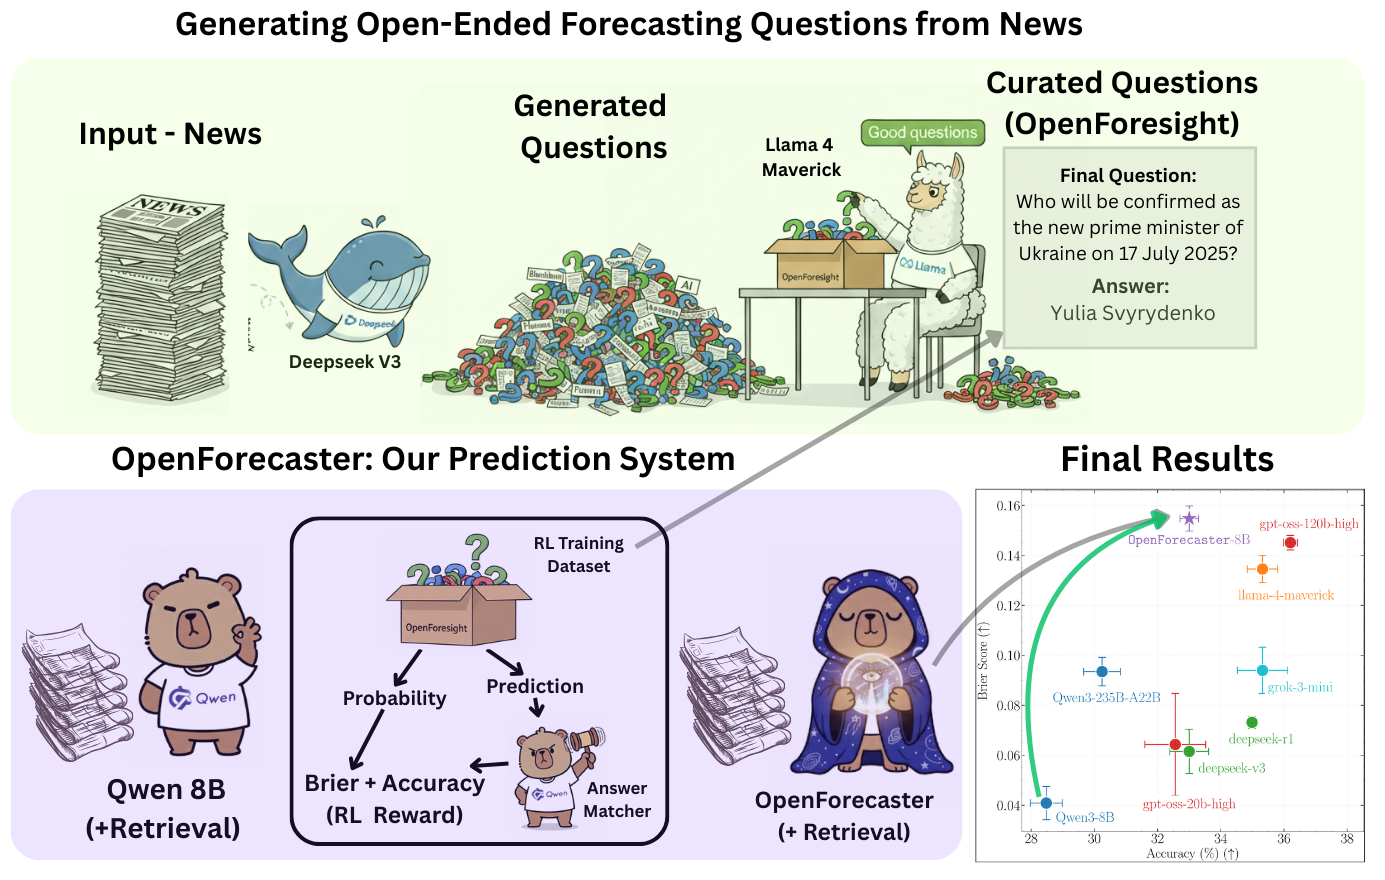
\includegraphics[width=0.9\linewidth]{figures/fig1preview.png}
    \vspace{-0.2cm}
    \caption{A summary of our methodology for training language model forecasters.}
    \label{fig:fig1}
    \vspace{-0.5cm}
\end{figure}

\looseness -1 \textbf{Final results}. In \Cref{sec:results}, we report results on our held-out test set of open-ended forecasting questions from May to August 2025, and FutureX~\citep{zeng2025futurex}, an external forecasting benchmark. RL training on \ourdataset \ makes the predictions of our specialized 8B model competitive with much larger proprietary models in both accuracy and calibration. We also observe large improvements on consistency evaluations for long-term predictions~\citep{paleka2025consistency}. Finally, we find calibration from our forecasting training generalizes to multiple out of distribution benchmarks. \vspace{0.15cm}

By providing rigorous probabilistic predictions, open-ended forecasting systems could transform policy making, corporate planning, and financial risk management~\citep{tetlock2017expert}. To promote forecasting research, we open-source our dataset, code, and models.